\nonstopmode

\documentclass[letterpaper,11pt,titlepage]{article}
\usepackage{amsthm,amssymb,mathtools}
\mathtoolsset{showonlyrefs}
\usepackage{bm}
\usepackage[margin=1in]{geometry}
\usepackage{booktabs}
\usepackage{enumitem}
\usepackage{framed}
\usepackage{tikz}
\usetikzlibrary{shapes,arrows,positioning,patterns,calc}
\usepackage{pgfplots}
\pgfplotsset{compat=1.9}
\usepackage{listings}
\usepackage[numbered,framed]{mcode}

\usepackage{fancyhdr}
\pagestyle{fancy}
\fancyhead{}
\fancyfoot{}
\fancyfoot[L]{K.\ Okkelberg}
\fancyfoot[R]{\thepage}
\renewcommand{\headrulewidth}{0pt}
\renewcommand{\footrulewidth}{0.5pt}

\newcommand*\dif{\mathop{}\!\mathrm{d}}
\newcommand{\trans}{^\text{T}}
\newcommand{\herm}{^\text{H}}
\DeclareMathOperator{\E}{E}
\DeclareMathOperator{\trace}{trace}
\DeclareMathOperator{\sign}{sign}
\let\Pr\relax
\DeclareMathOperator{\Pr}{P}
\newcommand*\pder[2]{\frac{\partial #1}{\partial #2}}
\newcommand*\R{\mathbb{R}}

\tikzstyle{line} = [draw,>=latex]
\tikzstyle{dot} = [circle,fill=black,inner sep=0pt,minimum size=4pt]

\begin{document}

\title{ECE 6553: Homework \#2}
\author{Klaus Okkelberg}
\date{February 16, 2017}
\maketitle

\setlist{listparindent=\parindent}

\begin{enumerate}[leftmargin=0pt]

\item
  \begin{enumerate}
  \item Since $\tau$ and $x_0$ are given, $x(t)$ is fixed for $0\le t<\tau$. Thus, the cost only depends on the integral from $\tau$ to $T$:
    \[ J(\rho) = \int_0^T\! L(x(t))\dif t = \int_0^\tau\! L(x(t))\dif t + \int_\tau^T\! L(x(t))\dif t = C + \int_\tau^T\! L(x(t))\dif t, \]
    since the finite jump $\rho$ in $x(\tau)$ does not affect the integral. In essence, we are finding the optimal initial condition at time $\tau$, i.e. $x(\tau^+)$. The Lagrangian is
    \[ \tilde J(\rho) = C + \int_\tau^T\! \Big\{ L(x(t)) + \lambda\trans(t)[f(x(t))-\dot x(t)] \Big\} \dif t \]
    Perturbing $\rho$ as $\rho\mapsto\rho+\varepsilon\nu$ causes a variation in $x(t)\mapsto x(t)+\varepsilon\eta(t)$:
    \begin{align}
      \tilde J(\rho+\varepsilon\nu) &= C + \int_\tau^T\! \Big\{ L(x(t)+\varepsilon\eta(t)) + \lambda\trans(t)[f(x(t)+\varepsilon\eta(t))-\dot x(t)-\varepsilon\dot\eta(t)] \Big\} \dif t + o(\varepsilon) \\[-3ex]
                                    &= C + \int_\tau^T\! \left\{ L(x) + \varepsilon\pder{L}{x}(x)\eta  + \lambda\trans\left[f(x) + \varepsilon\pder{f}{x}(x)\eta -\dot x -\varepsilon\dot\eta\right] \right\} \dif t + o(\varepsilon) \\
      \tilde J(\rho+\varepsilon\nu) - \tilde J(\rho) &= \int_\tau^T\! \left\{ \varepsilon\pder{L}{x}(x)\eta  + \lambda\trans\left[\varepsilon\pder{f}{x}(x)\eta  -\varepsilon\dot\eta\right] \right\} \dif t + o(\varepsilon) \\
      \delta \tilde J(\rho;\nu) &=  \int_\tau^T\! \left[ \pder{L}{x}(x)\eta  + \lambda\trans \pder{f}{x}(x)\eta \right] \dif t - \int_\tau^T\! \lambda\trans\dot\eta \dif t \\
                                    &=  \int_\tau^T\! \left[ \pder{L}{x}(x)\eta  + \lambda\trans \pder{f}{x}(x)\eta \right] \dif t + \int_\tau^T\! \dot\lambda\trans\eta \dif t - \lambda\trans(T)\eta(T) + \lambda\trans(\tau)\eta(\tau) \\
                                    &=  \int_\tau^T\! \left[ \pder{L}{x}(x)  + \lambda\trans \pder{f}{x}(x) + \dot\lambda\trans \right]\eta \dif t - \lambda\trans(T)\eta(T) + \lambda\trans(\tau)\eta(\tau)
    \end{align}
    We want the directional derivative to be 0, so we pick
    \begin{equation}
      \begin{dcases}
        \dot\lambda(t) = - \pder{L\trans}{x}(x(t)) - \pder{f\trans}{x}(x(t)) \lambda(t) \\
        \lambda(T) = 0
      \end{dcases}
      \label{eq:1a}
    \end{equation}
    This gives
    \[
      \delta \tilde J(\rho;\nu) = \pder{\tilde J}{\rho}\nu = \lambda\trans(\tau) \eta(\tau) = \lambda\trans(\tau) \nu.
    \]
    This is linear in $\nu$ so the FONC is
    \[
      \pder{\tilde J}{\rho} = \lambda(\tau) = 0,
    \]
    where $\lambda(t)$ satisfies \eqref{eq:1a}.

  \item Now, we perturb $\rho=\alpha w\mapsto (\alpha+\varepsilon)w=\alpha w+\varepsilon\nu$, where $w=\nu$. This causes a variation in $x(t)\mapsto x(t)+\varepsilon\eta(t)$, as before. However, the directional derivative only has to be 0 along $\nu=w$ instead of for all $\nu\in\R^n$. Thus, the FONC is
    \[
      \delta \tilde J(\rho;\nu) = \lambda\trans(\tau) w = 0.
    \]
    The $\lambda(\tau)\in\R^n$ that satisfy this condition are vectors that lie in the hyperplane perpendicular to $w$, of which there are infinitely many. $\lambda(t)$ still has to satisfy \eqref{eq:1a}.
  \end{enumerate}
  \clearpage

\item \begin{enumerate}
  \item The thick line in the figure indicates the portion where $x(t)=\hat x(t)$, $0\le t<\tau$. The thin solid line is the original trajectory $x$, and the dashed line is the perturbed trajectory $\hat x$. The vertical lines with arrowheads indicate the state jumps.

    \begin{center}
      \begin{tikzpicture}[scale=1.5]
        \draw [thick,->] (-0.5,0) -- (6,0) node [anchor=west] {$t$};
        \draw [thick,->] (0,-0.5) -- (0,4);
        \draw [thick] (5.5,0.2) -- (5.5,-0.2) node [anchor=north] {$T$};
        \draw [thick] (2,0.2) -- (2,-0.2) node [anchor=north] {$\tau\vphantom{\theta}$};
        \draw [thick] (2.75,0.2) -- (2.75,-0.2) node [anchor=north] {$\tau+\varepsilon\theta$};
        \draw [thick] (0.2,2) -- (-0.2,2) node [anchor=east] {$x_0$};
        \node [anchor=north east] at (0,0) {$0$};
        \draw [ultra thick] (0,2) .. controls (0.6,1) and (0.9,2.5) .. (2,2) coordinate (a);
        \node [anchor=south] at (1,2.2) {$x=\hat x$};
        \draw [thin] ($(a)+(0,-0.5)$) coordinate (b) .. controls (3,0) and (4.5,3) .. (5.5,2) node [anchor=west] {$x$};
        \draw [-latex,thin] (a) -- (b) node [anchor=east] {$\rho$};
        \draw [dashed,thick] (a) .. controls (2.5,1.6) .. (2.75,1.7) coordinate (c);
        \draw [dashed,thick] ($(c)+(0,0.35)$) coordinate (d) .. controls (3.5,3) and (4.5,3.5) .. (5.5,3) node [anchor=west] {$\hat x$};
        \draw [dashed,thick,-latex] (c) -- (d) node [anchor=west] {$\rho+\varepsilon\nu$};
      \end{tikzpicture}
    \end{center}

  \item Yes, direct application of Calculus of Variations would run into trouble. So far in class, we have only considered one perturbation. However, here both $\rho$ and $\tau$ are being perturbed. This means there are two changes in trajectory, i.e.\ $\hat x(t)=x(t)+\varepsilon\eta_1(t)+\varepsilon\eta_2(t)+o(\varepsilon)$.

    The FONCs for both perturbations can be computed using Calculus of Variations, but there would be two equations constraining the costate, one from each directional derivative. This means the costate is likely overconstrained and not solvable.
  \end{enumerate}

\item \begin{enumerate}
  \item The Lagrangian is
    \[
      \tilde J(\tau) = \int_0^\tau\! \big[ L(x(t)) + \lambda\trans(t) (-\alpha-\dot x) \big] \dif t + \int_\tau^1\! \big[ L(x(t)) + \lambda\trans(t) (\alpha-\dot x) \big] \dif t
    \]
    Perturbing $\tau\mapsto \tau+\varepsilon\theta$ causes $x(t)\mapsto x(t)+\varepsilon\eta(t)$. Note that $\eta=\dot \eta=0$ on $[0,\tau)$.
    \begin{align}
      \tilde J(\tau+\varepsilon\theta) &= \int_0^\tau\! \left\{ L(x) + \lambda\trans [-\alpha-\dot x] \right\} \dif t \\
                                       & \qquad + \int_\tau^{\tau+\varepsilon\theta}\! \left\{ L(x+\varepsilon\eta) + \lambda\trans [-\alpha - \dot x - \varepsilon\dot\eta] \right\} \dif t \\
                                       & \qquad + \int_{\tau+\varepsilon\theta}^1\! \left\{ L(x+\varepsilon\eta) + \lambda\trans [\alpha - \dot x - \varepsilon\dot\eta] \right\} \dif t + o(\varepsilon) \\
                                       &= \int_0^\tau\! \left\{ L(x) + \lambda\trans [-\alpha-\dot x] \right\} \dif t \\
                                       & \qquad + \int_\tau^{\tau+\varepsilon\theta}\! \left\{ L(x) + \varepsilon\pder{L}{x}(x)\eta + \lambda\trans [-\alpha - \dot x - \varepsilon\dot\eta] \right\} \dif t \\
                                       & \qquad + \int_{\tau+\varepsilon\theta}^1\! \left\{ L(x) +\varepsilon\pder{L}{x}(x)\eta + \lambda\trans [\alpha - \dot x - \varepsilon\dot\eta] \right\} \dif t + o(\varepsilon) \displaybreak \\
      \tilde J(\tau+\varepsilon\theta) - \tilde J(\tau) &= \underbrace{ \int_\tau^{\tau+\varepsilon\theta}\! \left\{ \varepsilon\pder{L}{x}(x)\eta + \lambda\trans [-\alpha - \alpha - \varepsilon\dot\eta] \right\} \dif t }_{\displaystyle I_1} \label{eq:3a} \\
                                       & \qquad + \underbrace{ \int_{\tau+\varepsilon\theta}^1\! \left\{ \varepsilon\pder{L}{x}(x)\eta + \lambda\trans [- \varepsilon\dot\eta] \right\} \dif t }_{\displaystyle I_2} + o(\varepsilon)
    \end{align}
    Using the mean-value theorem, the first integral is
    \begin{align}
      I_1 &= \int_\tau^{\tau+\varepsilon\theta}\! \left\{ \varepsilon\pder{L}{x}(x)\eta - \lambda\trans [2\alpha + \varepsilon\dot\eta] \right\} \dif t \\
          &= [(\tau+\varepsilon\theta)-\tau] \cdot [-2\lambda\trans(\xi)\alpha] + o(\varepsilon) \\
          &= -2 \varepsilon\theta \lambda\trans(\xi)\alpha + o(\varepsilon) \label{eq:3a_i1}
    \end{align}
    where $\tau\le\xi\le\tau+\varepsilon\theta$. The second integral is
    \begin{align}
      I_2 &= \int_{\tau}^1\! \left\{ \varepsilon\pder{L}{x}(x)\eta - \varepsilon \lambda\trans \dot\eta \right\} \dif t - \underbrace{ \int_\tau^{\tau+\varepsilon\theta}\! \left\{ \varepsilon\pder{L}{x}(x)\eta + \lambda\trans [- \varepsilon\dot\eta] \right\} \dif t }_{o(\varepsilon)} \\
          &= \varepsilon \int_{\tau}^1\! \left[ \pder{L}{x}(x)\eta + \dot\lambda\trans\eta \right] \dif t - \varepsilon \lambda\trans(1)\eta(1) + \varepsilon \lambda\trans(\tau) \underbracket{\eta(\tau)}_{=0} + o(\varepsilon) \\
          &= \varepsilon \int_{\tau}^1\! \left[ \pder{L}{x}(x) + \dot\lambda\trans \right] \eta \dif t - \varepsilon \lambda\trans(1)\eta(1) + o(\varepsilon) \label{eq:3a_i2}
    \end{align}
    Substituting \eqref{eq:3a_i1} and \eqref{eq:3a_i2} into \eqref{eq:3a} produces
    \begin{align}
      \tilde J(\tau+\varepsilon\theta) - \tilde J(\tau) &= -2 \varepsilon\theta \lambda\trans(\xi)\alpha + \varepsilon \int_{\tau}^1\! \left[ \pder{L}{x}(x) + \dot\lambda\trans \right] \eta \dif t - \varepsilon \lambda\trans(1)\eta(1) + o(\varepsilon) \\
      \delta \tilde J(\tau;\theta) &= \lim_{\varepsilon\to0} \frac{\tilde J(\tau+\varepsilon\theta)-\tilde J(\tau)}{\varepsilon} \\
                                                        &= -2 \theta \lambda\trans(\tau)\alpha +  \int_{\tau}^1\! \left[ \pder{L}{x}(x) + \dot\lambda\trans \right] \eta \dif t -  \lambda\trans(1)\eta(1) ,
    \end{align}
    since $\xi\to\tau$ as $\varepsilon\to0$. Select the costate such that
    \[
      \begin{dcases}
        \dot\lambda(t) = -\pder{L}{x}(x(t)) = -\pder{}{x} \frac{1}{2} (x(t)-\alpha)^2 = \alpha-x(t) \\
        \lambda(1) = 0
      \end{dcases}
    \]
    With this choice of $\lambda(t)$,
    \begin{align}
      \delta \tilde J(\tau;\theta) &= -2\alpha\lambda(\tau) \theta = \pder{\tilde J}{\tau} \theta \\
      \pder{\tilde J}{\tau} &= -2\alpha\lambda(\tau) = 0 \\
      \lambda(\tau) &= 0
    \end{align}
    From the dynamics of $x$,
    \[
      x(t) = \begin{cases}
        -\alpha t + 1, & t\in[0,\tau) \\
        \alpha (t-\tau) - \alpha \tau + 1, & t\in[\tau,1]
      \end{cases}
    \]
    By the fundamental theorem of calculus,
    \begin{align}
      \lambda(1)-\lambda(\tau) &= \int_\tau^1\! \dot\lambda(t)\dif t = \int_\tau^1\! [\alpha-x(t)] \dif t \\
                               &= \int_\tau^1\! [\alpha - \alpha(t-\tau) + \alpha\tau - 1] \dif t \\
                               &= \bigg[ -\frac{1}{2} \alpha t^2 + (\alpha+2\alpha\tau-1)t \bigg]_\tau^1 \\
                               &= -\frac{1}{2} \alpha (1-\tau^2) + (\alpha+2\alpha\tau-1)(1-\tau) \\
                               &= (1-\tau) \left[ -\frac{\alpha}{2}(1+\tau) + \alpha + 2\alpha\tau - 1 \right] \\
                               &= (1-\tau) \left[ \frac{\alpha}{2} - 1 + \left( \frac{3\alpha}{2} \right) \tau \right]
    \end{align}
    Since $\lambda(1)-\lambda(\tau)=0-0=0$, the optimal $\tau$ is given by the zeros of the expression, i.e. $\tau=1$ or $\tau=(2-\alpha)/3\alpha$. Since we need $\tau\le1$,
    \[
      \tau^* = \begin{dcases}
        \frac{2-\alpha}{3\alpha}, & \alpha\ge\frac{1}{2} \\
        1, & \alpha < \frac{1}{2}
      \end{dcases}
    \]

  \item The optimal switching times and the costs are shown in the table below.
    \begin{center}
      \begin{tabular}{ccc}
        \toprule
        $\alpha$ & $\tau^*$ & $J(\tau^*)$ \\
        \midrule
        0.25 & 1 & 19/96 \\
        1 & 1/3 & 1/54 \\
        1.75 & 1/21 & 757/6048 \\
        \bottomrule
      \end{tabular}
    \end{center}
    The costs were calculuated as follows:
    \begin{align}
      \alpha=0.25 \Longrightarrow J(1) &= \int_0^1\! \frac{1}{2} (-0.25t+1-0.25)^2 \dif t \\
                                       &= \left. - \frac{1}{6\cdot0.75} (-0.25t + 0.75)^3 \right|_0^1 \\
                                       &= -\frac{1}{6\cdot0.25} \big[ (-0.25+0.75)^3 - (0.75)^3 \big] \\
                                       &= \frac{19}{96} \approx 0.1979 \displaybreak \\
      \alpha=1 \Longrightarrow J(1/3) &= \int_0^{1/3}\! \frac{1}{2} (-t+1-1)^2 \dif t + \int_{1/3}^1 \frac{1}{2} \left( t-\frac{1}{3} - \frac{1}{3} + 1 - 1 \right)^2 \dif t \\
                                       &= \left. \frac{1}{6} t^3 \right|_0^{1/3} + \left. \frac{1}{6} \left(t-\frac{2}{3}\right)^3 \right|_{1/3}^1 = \frac{1}{6} \left[ \frac{1}{3^3} + \frac{1}{3^3} + \frac{1}{3^3} \right] \\
                                       &= \frac{1}{54} \approx 0.01852 \\
      \alpha=1.75 \Longrightarrow J(1/21) &= \int_0^{1/21} \frac{1}{2} (-1.75t+1-1.75)^2 \dif t \\
                                       &\qquad + \int_{1/21}^1 \frac{1}{2} \left[ 1.75\left(t-\frac{1}{21}\right) - \frac{1.75}{21} + 1 - 1.75 \right]^2 \dif t \\
                                       &= \left. - \frac{1}{6\cdot1.75} (-1.75t-0.75)^3 \right|_0^{1/21} + \left. \frac{1}{6\cdot1.75} \left( 1.75t - \frac{2(1.75)}{21} - 0.75 \right)^3 \right|_{1/21}^1 \\[-3ex]
                                       &= \frac{1}{6\cdot1.75} \left[ \left(\frac{1.75}{21}+0.75\right)^3 - 0.75^3 + \left( 1 - \frac{3.5}{21} \right)^3 - \left( -\frac{1.75}{21} - 0.75 \right)^3 \right] \\[-2ex]
                                       &= \frac{757}{6048} \approx 0.1252
    \end{align}
    The following figure shows the plots and approximate costs from Matlab. We can see that the costs calculated by Matlab are close to the actual costs calculated by hand.
    \begin{center}
      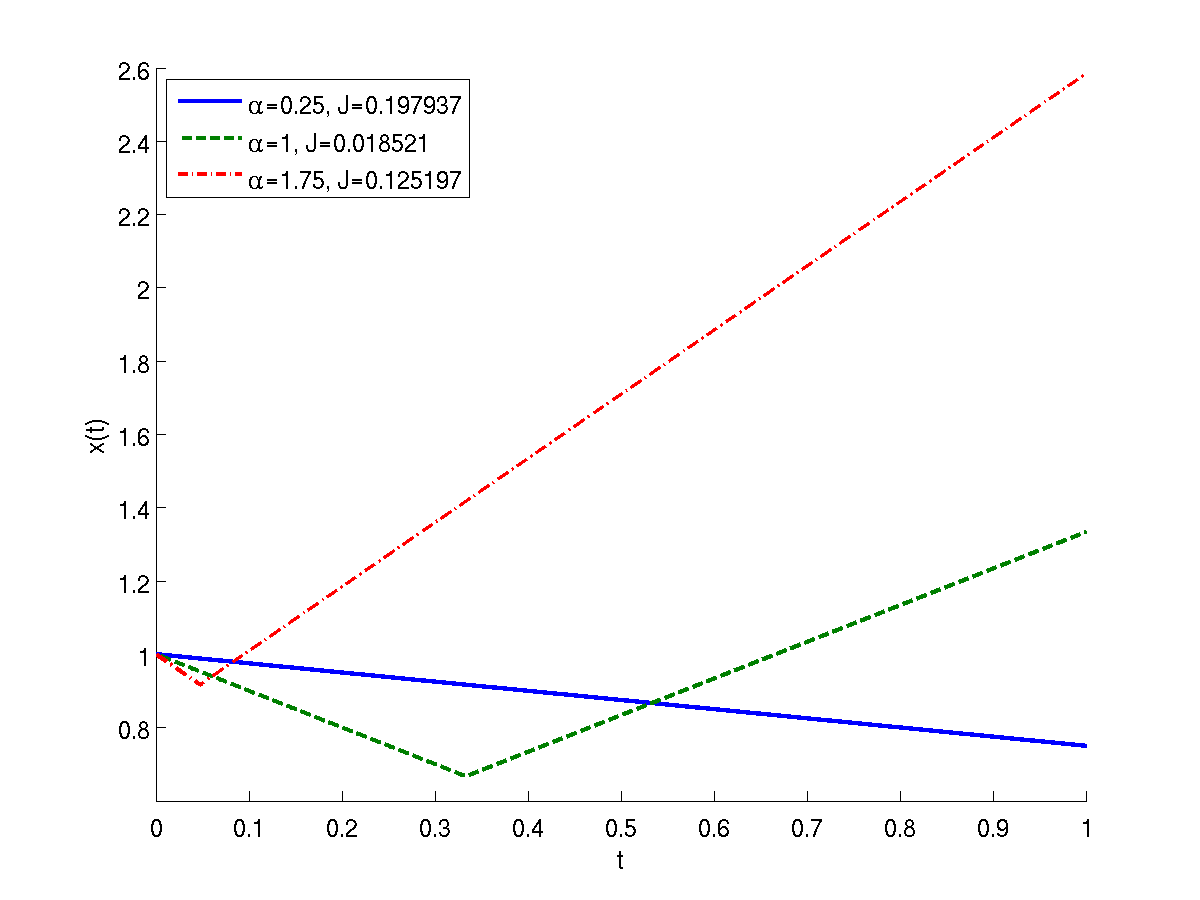
\includegraphics[width=0.8\textwidth]{hw2p3b}
    \end{center}
    \clearpage
    \lstinputlisting{hw2p3.m}
  \end{enumerate}
  \clearpage

\item \begin{enumerate}
  \item As shown in class, the costate equation only depends on the partial derivative of the Hamiltonian with respect to $x(t)$. The fact that the control is $x_0$ does not matter. Therefore, the costate has to satisfy
    \begin{align}
      \dot\lambda &= -\pder{H\trans}{x} = -\pder{L\trans}{x} - \pder{f\trans}{x} \lambda \\
                  &= - \left( \pder{}{x} \frac{1}{2} x\trans Qx \right)\trans - \left( \pder{}{x} Ax \right)\trans \lambda \\
                  &= - Qx - A\trans \lambda \\
      \lambda(T) &= \pder{\Psi\trans}{x} = 0 \\
      \Longrightarrow & \begin{cases}
        \dot\lambda =  -Qx - A\trans \lambda \\
        \lambda(T) = 0
      \end{cases}
    \end{align}
  \item A Hurwitz matrix is defined as a square matrix whose eigenvalues have strictly negative real parts. From the dynamics of $\dot\lambda$, we see that the costate is governed by $-A\trans$, whose eigenvalues would have strictly positive real parts, since eigenvalues are given by
    \[
      0 = \det(A-\lambda I) = -\det(-(A-\lambda I)\trans) = -\det(-A\trans-(-\lambda)I)
    \]
    Therefore, the costate equation is unstable.
  \item Since the costate equation is unstable, we need certain $-Qx$ to stabilize the system in order to satisfy the boundary condition $\lambda(0)=0$. However, this is untrue for general $x$. Therefore, the numerical solution to this problem is sensitive to the inital $x_{0,0}$. This means the solution is not robust to the inital point chosen. Additionally, the gradient $\lambda(0)$ is likely to be large due to the instability, so the costate converges quickly for certain initial $x_{0,0}$. This means the numerical solution can be very efficient.
  \end{enumerate}

\item This problem is equivalent to the following unconstrained optimization problem, where the constraint has been substituted into the utility function:
  \[
    \max_{T,c} F(T,c) = \gamma (T+c) - \frac12 \alpha T^2 - \frac12 \beta c^2
  \]
  The FONCs are
  \begin{align}
    \pder{F}{T} &= \gamma - \alpha T = 0 \Longrightarrow T = \frac{\gamma}{\alpha} \\
    \pder{F}{c} &= \gamma - \beta c = 0 \Longrightarrow c = \frac{\gamma}{\beta}
  \end{align}
  For this to be a maximum instead of a minimum, it is sufficient that the Hessian is negative definite:
  \[
    \begin{bmatrix}
      \displaystyle \pder{^2 F}{T^2} & \displaystyle \pder{^2 F}{T\partial c} \\[2ex]
      \displaystyle \pder{^2 F}{c\partial T} & \displaystyle \pder{^2 F}{c^2}
    \end{bmatrix} = \begin{bmatrix}
      -\alpha & 0 \\ 0 & -\beta
    \end{bmatrix} \prec 0,
  \]
  since the Hessian is Hermitian and has strictly negative eigenvalues. Therefore, the optimal grade is
  \[
    g^* = \gamma(T+c) = \gamma \left( \frac{\gamma}{\alpha} + \frac{\gamma}{\beta} \right) = \gamma^2 \left( \frac{\alpha+\beta}{\alpha\beta} \right)
  \]

\item The augmented cost is
  \[
    \tilde J(u) = \int_0^T\! \left[ L(x,u,t) + \lambda\trans \Phi(x,u,t) \right] \dif t
  \]
  Consider a perturbation $u\mapsto u+\varepsilon\nu$ that causes a change $x\mapsto x+\varepsilon\eta$:
  \begin{align}
    \tilde J(u+\varepsilon\nu) &= \int_0^T\! \left[ L(x+\varepsilon\eta,u+\varepsilon\nu,t) + \lambda\trans \Phi(x+\varepsilon\eta,u+\varepsilon\nu,t) \right] \dif t \\
                               &= \int_0^T\! \bigg\{ L(x,u,t) + \varepsilon\pder{L}{x}(x,u,t)\eta + \varepsilon\pder{L}{u}(x,u,t)\nu \\
                               & \qquad + \lambda\trans \left[ \Phi(x,u,t) + \varepsilon\pder{\Phi}{x}(x,u,t)\eta + \varepsilon\pder{\Phi}{u}(x,u,t)\nu \right] \bigg\} \dif t + o(\varepsilon) \\
    \tilde J(u+\varepsilon\nu) - \tilde J(u) &= \int_0^T\! \bigg\{ \varepsilon\pder{L}{x}(x,u,t)\eta + \varepsilon\pder{L}{u}(x,u,t)\nu \\
                               & \qquad + \lambda\trans \left[ \varepsilon\pder{\Phi}{x}(x,u,t)\eta + \varepsilon\pder{\Phi}{u}(x,u,t)\nu \right] \bigg\} \dif t + o(\varepsilon) \\
    \delta \tilde J(u;\nu) &= \int_0^T\! \bigg\{ \pder{L}{x}(x,u,t)\eta + \pder{L}{u}(x,u,t)\nu + \lambda\trans \left[ \pder{\Phi}{x}(x,u,t)\eta + \pder{\Phi}{u}(x,u,t)\nu \right] \bigg\} \dif t \\
                               &= \int_0^T\! \left[ \pder{L}{u}(x,u,t) + \lambda\trans \pder{\Phi}{u}(x,u,t) \right] \nu\dif t + \int_0^T\! \left[ \pder{L}{x}(x,u,t) + \lambda\trans \pder{\Phi}{x}(x,u,t) \right] \eta\dif t \\[-7ex]
  \end{align}
  Since for optimality, we want $\delta\tilde J(u;\nu)=0$ for all $\nu$ and $\eta$, we need
  \[
    \begin{dcases}
      \pder{L}{u}(x,u,t) + \lambda\trans \pder{\Phi}{u}(x,u,t) = 0, & \forall t\in[0,T] \\
      \pder{L}{x}(x,u,t) + \lambda\trans \pder{\Phi}{x}(x,u,t) = 0, & \forall t\in[0,T]
    \end{dcases}
  \]

\end{enumerate}

\end{document}
